
\begin{figure}[h!]
\fbox{
\begin{minipage}{\textwidth}\centering
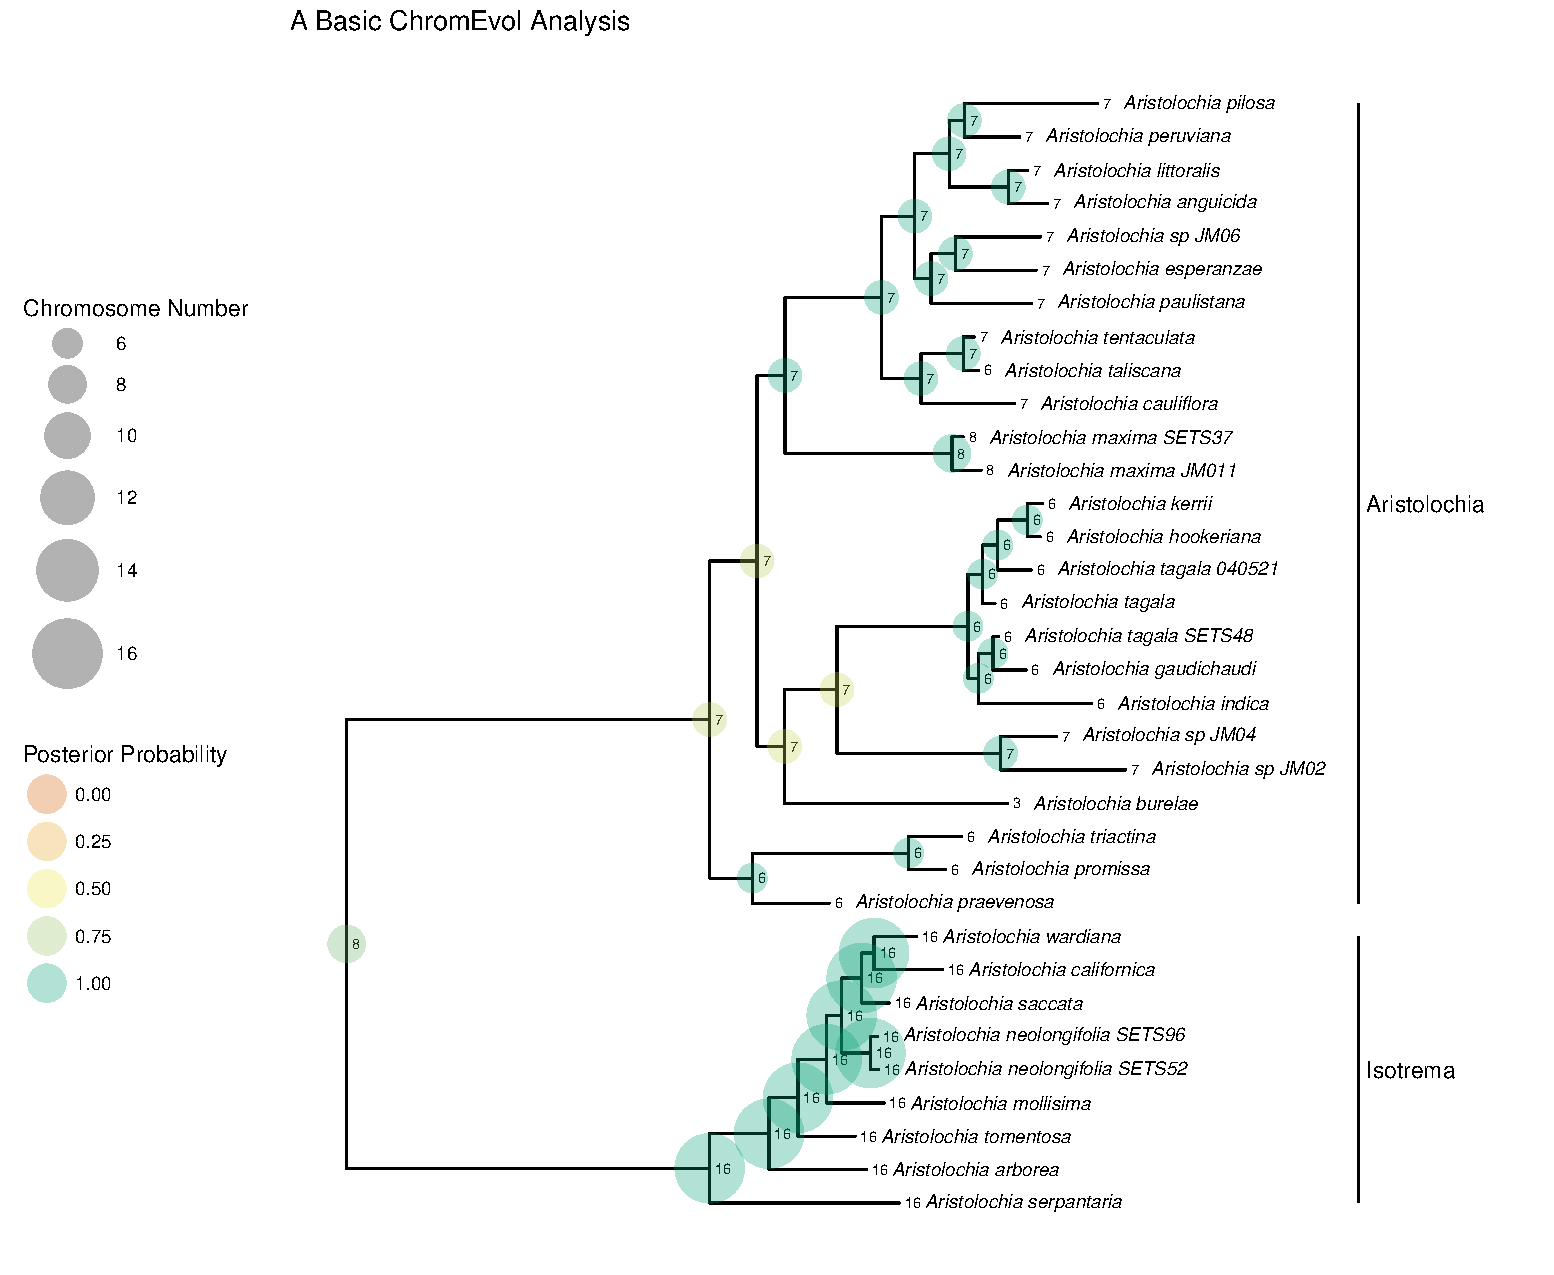
\includegraphics[width=0.92\textwidth,angle=0]{\ResourcePath figures/ChromEvol_simple}
\caption{\small Maximum a posteriori ancestral chromosome number estimates for \textit{Aristolochia}
    inferred using \RevBayes and plotted using the \RevGadgets R package.
    Section \ref{sec:chromo_basic_analysis} describes how to perform this analysis.}
\end{minipage}}
\label{fig:chromevol_simple}
\end{figure}

\section{Example: A Simple ChromEvol Analysis}\label{sec:chromo_basic_analysis}

In this example, we will use molecular sequence data and chromosome counts from \citet{ohi2006molecular} of the plant genus \textit{Aristolochia} (commonly called Dutchman's pipe plants). 
We will use a simple ChromEvol model to infer rates of chromosome evolution and ancestral chromosome numbers.

\medskip
\subsection{Tutorial Format}\label{subsect:Exercise-Format}

This tutorial follows a specific format for issuing instructions and information.

{\begin{framed}
The boxed instructions guide you to complete tasks that are not part of the \RevBayes syntax, but rather direct you to create directories or files or similar.
\end{framed}}


Information describing the commands and instructions will be written in paragraph-form before or after they are issued.

All command-line text, including all \Rev syntax, are given in \cl{monotype font}. 
Furthermore, blocks of \Rev code that are needed to build the model, specify the analysis, or execute the run are given in separate shaded boxes.
For example, we will instruct you to create a constant node called \cl{example} that is equal to \cl{1.0} using the \cl{<-} operator like this:
{\tt \begin{snugshade*}
\begin{lstlisting}
example <- 1.0
\end{lstlisting}
\end{snugshade*}
}

It is important to be aware that some PDF viewers may render some characters given as \colorbox{shadecolor}{\tt{Rev commands}} differently. 
Thus, if you copy and paste text from this PDF, you may introduce some incorrect characters. 
Because of this, we recommend that you type the instructions in this tutorial or copy them from the scripts provided. 


\medskip
\subsection{Data and Files}\label{subsect:Exercise-DataFiles}

{\begin{framed}
On your own computer, create a directory called {\textcolor{red}{\cl{RB\_Chromosome\_Evolution\_Tutorial}}} (or any name you like). 

In this directory download and unzip the archive containing the data files: \href{http://rawgit.com/revbayes/revbayes_tutorial/master/RB_Chromosome_Evolution_Tutorial/data.zip}{\cl{data.zip}}.

This will create a folder called \cl{data} that contains the files necessary to complete this exercise.

\end{framed}}


\bigskip
\subsection{Creating the \Rev File}\label{subsect:Exercise-CreatingFiles}

{\begin{framed}
Create a new directory (in \cl{RB\_Chromosome\_Evolution\_Tutorial}) called {\textcolor{red}{\cl{scripts}}}. (If you do not have this folder, please refer to the directions in section \ref{subsect:Exercise-DataFiles}.)
\end{framed}}

When you execute \RevBayes in this exercise, you should do so within the main directory you created (\cl{RB\_Chromosome\_Evolution\_Tutorial}), thus, if you are using a Unix-based operating system, we recommend that you add the \RevBayes binary to your path.
\bigskip

For complex models and analyses, it is best to create \Rev script files that will contain all of the model parameters, moves, and functions. 
In this first section, you will create a file called \textcolor{red}{\texttt{ChromEvol\_simple.Rev}} from scratch and save it in the \cl{scripts} directory.

The full scripts for these examples are also provided in the \RevBayes tutorial repository\footnote{\url{http://rawgit.com/revbayes/revbayes_tutorial/master/RB_Chromosome_Evolution_Tutorial/scripts.zip}}. 
Please refer to these files to verify or troubleshoot your own scripts. 

{\begin{framed}
Open your text editor and create the master \Rev file called {\textcolor{red}{\texttt{ChromEvol\_simple.Rev}}} in the \cl{scripts} directory.

Enter the \Rev code provided in this section into this file.
\end{framed}}

The file you will begin in this section will be the one you load into \RevBayes when you've completed all of the components of the analysis. The file will contain the \Rev code to load the data files, set up the model, run the MCMC analysis, and summarize the results.

\medskip
\subsection{Reading in Data}\label{subsub:Exercise-LoadData}

First, we'll read in the phylogeny. In this example the phylogeny is assumed known. In further
examples we'll jointly estimate chromosome evolution and the phylogeny.
{\tt \begin{snugshade*}
\begin{lstlisting}
phylogeny <- readBranchLengthTrees("data/aristolochia.tree")[1]
\end{lstlisting}
\end{snugshade*}}

We need to limit the maximum number of chromosomes allowed in our model,
so here we use the largest observed chromosome count plus 10. This is an arbitrary limit
on the size of the state space that could be increased if necessary.
{\tt \begin{snugshade*}
\begin{lstlisting}
max_chromo = 26 
\end{lstlisting}
\end{snugshade*}}

Now we get the observed chromosome counts from a tab-delimited file.
{\tt \begin{snugshade*}
\begin{lstlisting}
chromo_data = readCharacterDataDelimited("data/aristolochia_chromosome_counts.tsv", stateLabels=(max_chromo + 1), type="NaturalNumbers", delimiter="\t", headers=FALSE)
\end{lstlisting}
\end{snugshade*}}


\bigskip
\subsection{The Chromosome Evolution Model}


We'll use exponential priors with prior mean 0.1 to model the rates of polyploidy and 
dysploidy events along the branches of the phylogeny.
\texttt{gamma} is the rate of chromosome gains,
\texttt{delta} is the rate of chromosome losses, and
\texttt{rho} is the rate of polyploidization.
{\tt \begin{snugshade*}
\begin{lstlisting}
gamma ~ dnExponential(10.0)
delta ~ dnExponential(10.0)
rho ~ dnExponential(10.0)
\end{lstlisting}
\end{snugshade*}}

Add MCMC moves for each of the rates. 
{\tt \begin{snugshade*}
\begin{lstlisting}
mvi = 1
moves[mvi++] = mvScale(gamma, lambda=1, weight=1)
moves[mvi++] = mvScale(delta, lambda=1, weight=1)
moves[mvi++] = mvScale(rho, lambda=1, weight=1)
\end{lstlisting}
\end{snugshade*}}

Now we create the rate matrix for the chromosome evolution model.
Here we will use a simple ChromEvol model that includes
only the rate of chromosome gain, loss, and polyploidization.
{\tt \begin{snugshade*}
\begin{lstlisting}
Q := fnChromosomes(max_chromo, gamma, delta, rho)
\end{lstlisting}
\end{snugshade*}}

Parameters for demi-polyploidization and rate modifiers could also
be added at this step for more complex models. For example, we
could have included the rate of demi-polyploidization \texttt{eta} 
and rate modifiers like this:
{\tt \begin{snugshade*}
\begin{lstlisting}
Q := fnChromosomes(max_chromo, gamma, delta, rho, eta, gamma_l, delta_l)
\end{lstlisting}
\end{snugshade*}}

Here we assume an equal prior probability for the frequency of chromosome numbers at the root of the tree. 
This does not mean that the frequencies are actually equal, we just give it an equal prior probability.
Alternatively, we could have treated the root frequencies as a free variable and estimated them from the observed data. 
This approach will be illustrated in further examples.
{\tt \begin{snugshade*}
\begin{lstlisting}
root_frequencies := simplex(rep(1, max_chromo + 1))
\end{lstlisting}
\end{snugshade*}}

Finally, we
create the stochastic node for the chromosome evolution continuous-time Markov chain (CTMC).
We also clamp the observed chromosome count data to the CTMC.
{\tt \begin{snugshade*}
\begin{lstlisting}
chromo_ctmc ~ dnPhyloCTMC(Q=Q, tree=phylogeny, rootFreq=root_frequencies, type="NaturalNumbers")
chromo_ctmc.clamp(chromo_data)
\end{lstlisting}
\end{snugshade*}}

All of the components of the model are now specified,
so now we wrap it into a single model object.
{\tt \begin{snugshade*}
\begin{lstlisting}
mymodel = model(phylogeny)
\end{lstlisting}
\end{snugshade*}}


\subsection{Set Up the MCMC}\label{subsect:Exercise-CompleteMCMC}


The next important step for our master \Rev file is to specify the MCMC monitors.
For this, we create a vector called \cl{monitors} that will each output MCMC samples. 
First, a screen monitor that will output every 10 iterations:
{\tt \begin{snugshade*}
\begin{lstlisting}
monitors[1] = mnScreen(printgen=10)
\end{lstlisting}
\end{snugshade*}}

Next, an ancestral state monitor which will sample ancestral states and write them to a log file.
We could additionally use the \texttt{mnStochasticCharacterMap} monitor to sample
stochastic character maps of chromosome evolution (see the next section for an example).
{\tt \begin{snugshade*}
\begin{lstlisting}
monitors[2] = mnJointConditionalAncestralState(filename="output/ChromEvol_simple_anc_states.log", printgen=10, tree=phylogeny, ctmc=chromo_ctmc, type="NaturalNumbers")
\end{lstlisting}
\end{snugshade*}}

And another monitor for logging all the model parameters. This will generate a file that can be opened in \Tracer for checking MCMC convergence and parameter estimates.
{\tt \begin{snugshade*}
\begin{lstlisting}
monitors[3] = mnModel(filename="output/ChromEvol_simple_model.log", printgen=10)
\end{lstlisting}
\end{snugshade*}}

Now we set up the MCMC and include code to execute the analysis. In this example we set the chain length to \texttt{200}, however
for a real analysis you would want to run many more iterations and check for convergence.
{\tt \begin{snugshade*}
\begin{lstlisting}
mymcmc = mcmc(mymodel, monitors, moves)
mymcmc.run(200)
\end{lstlisting}
\end{snugshade*}}


\medskip
\subsection{Summarize Ancestral States}

Now we need to add \Rev code that will summarize the sampled ancestral chromosome
numbers. First, read in the ancestral state trace generated by the ancestral state
monitor during the MCMC analysis:
{\tt \begin{snugshade*}
\begin{lstlisting}
anc_state_trace = readAncestralStateTrace("output/ChromEvol_simple_anc_states.log")
\end{lstlisting}
\end{snugshade*}}

Finally, summarize the values from the traces over the phylogeny.
Here we do a marginal reconstruction of the ancestral states, discarding the first 25\% of samples
as burnin. This will produce the file \texttt{ChromEvol\_simple\_final.tree} that contains
the phylogeny along with estimated ancestral states. 
We can use that file with the \RevGadgets R package to generate a plot of the ancestral states.

{\tt \begin{snugshade*}
\begin{lstlisting}
ancestralStateTree(phylogeny, anc_state_trace, "output/ChromEvol_simple_final.tree", burnin=0.25, reconstruction="marginal")
\end{lstlisting}
\end{snugshade*}}
Note that we could also have calculated joint or conditional ancestral states instead of (or in
addition to) the marginal ancestral states.
If we had sampled stochastic character maps, we would summarize them with the \texttt{characterMapTree}
function.


And now quit \RevBayes:
{\tt \begin{snugshade*}
\begin{lstlisting}
q()
\end{lstlisting}
\end{snugshade*}}

{\begin{framed}
You made it! Be sure to save the file.
\end{framed}}

\bigskip
\subsection{Execute the \RevBayes Analysis}\label{subsect:Exercise-RunMCMC}

With all the parameters specified and all analysis components in place, you are now ready to run your analysis. 
The \Rev scripts you just created will all be used by \RevBayes and loaded in the appropriate order.

{\begin{framed}
Begin by running the \RevBayes executable. In Unix systems, type the following in your terminal (if the \RevBayes binary is in your path):

\colorbox{black}{\strut\hspace{1mm}\textcolor[rgb]{0,1,1}{\cl{rb scripts/ChromEvol\_simple.Rev}}\hspace{0.6\textwidth}}
\end{framed}}

Provided that you started \RevBayes from the correct directory (\cl{RB\_Chromsome\_Evolution\_Tutorial}) the analysis should now run. Alternatively, from within \RevBayes you could use the \cl{source()} function to feed \RevBayes your master script file:
{\tt \begin{snugshade*}
\begin{lstlisting}
source("scripts/ChromEvol_simple.Rev")
\end{lstlisting}
\end{snugshade*}}

This will execute the analysis and you should see output similar to this (though not the exact same values):


{\tiny{\tt \begin{snugshade*}
\begin{lstlisting}
RevBayes

Visit the website www.RevBayes.com for more information about RevBayes.

RevBayes is free software released under the GPL license, version 3. Type 'license()' for details.

To quit RevBayes type 'quit()' or 'q()'.


> source("scripts/ChromEvol_simple.Rev")
   Processing file "scripts/ChromEvol_simple.Rev"
   Attempting to read the contents of file "aristolochia.tree"
   Successfully read file

   Running MCMC simulation
   This simulation runs 1 independent replicate.
   The simulator uses 3 different moves in a random move schedule with 3 moves per iteration

Iter        |      Posterior   |     Likelihood   |          Prior   |    elapsed   |        ETA   |
----------------------------------------------------------------------------------------------------
0           |       -61.8458   |       -63.6701   |        1.82431   |   00:00:00   |   --:--:--   |
10          |       -59.8779   |       -60.1293   |       0.251464   |   00:00:02   |   --:--:--   |
20          |        -59.251   |       -55.6886   |       -3.56249   |   00:00:04   |   00:00:36   |
30          |       -60.1883   |       -53.1068   |       -7.08147   |   00:00:06   |   00:00:34   |
40          |       -61.1943   |       -52.6285   |       -8.56577   |   00:00:09   |   00:00:36   |
50          |       -60.7165   |       -54.7084   |       -6.00804   |   00:00:11   |   00:00:33   |

|*...
\end{lstlisting}
\end{snugshade*}}}

When the analysis is complete, \RevBayes will quit and you will have a new directory called \cl{output} that will contain all of the files you specified with the monitors (Sect.\ \ref{subsect:Exercise-CompleteMCMC}).

\subsection{Plotting the Results}

Now we will plot the results of the MCMC analysis using the \RevGadgets R package.
Start R and set your working directory to the \cl{RB\_Chromsome\_Evolution\_Tutorial}
directory. Now run the command
\colorbox{black}{\strut\hspace{1mm}\textcolor[rgb]{0,1,1}{\cl{source("scripts/plot\_ChromEvol\_simple.R")}}} to generate Figure \ref{fig:chromevol_simple} below. There are many options to customize
the look of the plot, for options take a look inside the R script.

\subsection{Next Steps}

There are many extensions to the basic ChromEvol analysis demonstrated here. In the next
section we will look at how to set up more complex chromosome number evolution analyses.

 

\newpage
